\documentclass{math201}

\usepackage[backref]{hyperref} 
\hypersetup{hidelinks}
\usepackage{bookmark}

% =============================================
% Part 0 信息
% =============================================

\mathsetup{
  % 学生姓名
  student = {},
  % 学号
  student-id = {},
  % 院系
  experiment = {CCS程序安装和使用初步},
  % 专业班级
  discipline = {集成2021391},
  % 日期
  date = {\today},
}

\begin{document}

% =============================================
% Part 1  封面
% =============================================

\makecover

% =============================================
% Part 2 主文档
% =============================================

\section{实验内容}

熟悉如何安装CCS6或更高版本的CCS、以及软件的使用方法。包括创建工程、添加文件、编译、调试等。

\section{实验步骤}

\subsection{安装CCS6软件}

\begin{figure}[H]  
    \centering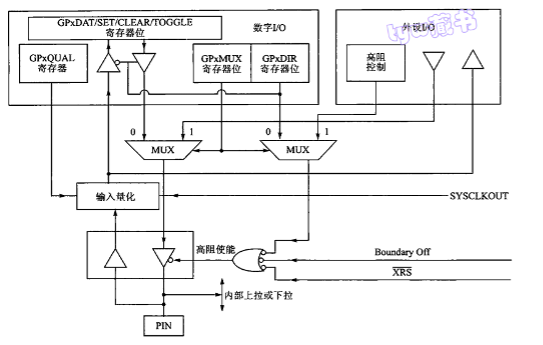
\includegraphics[width=0.8\linewidth]{Picture1.jpg}  
    \caption{安装类型选择 Custom Installation}
\end{figure}

\begin{figure}[H]  
  \centering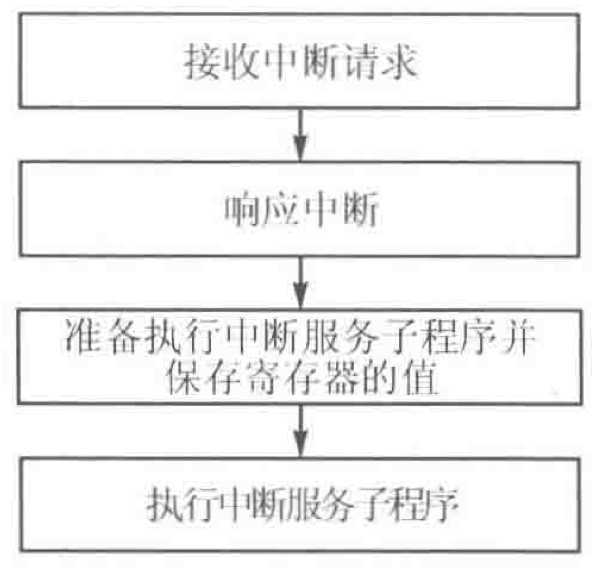
\includegraphics[width=0.8\linewidth]{Picture2.jpg}  
  \caption{在Select Components页面中必需选择`C2000 real-time MCUs`。}     
\end{figure}

\subsection{新建工程,添加文件、设置工程属性}

\begin{figure}[H]  
  \centering\includegraphics[width=0.8\linewidth]{Picture3.jpg}  
  \caption{新建项目,选择TMS320F2812}     
\end{figure}

\begin{figure}[H]  
  \centering\includegraphics[width=0.8\linewidth]{Picture4.jpg}  
  \caption{Include option中添加include文件夹路径}     
\end{figure}

\subsection{编译、下载程序}

main.c

\inputminted[
    frame=lines,
    framesep=2mm,
    baselinestretch=1.2,
    fontsize=\small,
    linenos
]{C}{code/main.c}

\begin{figure}[H]  
  \centering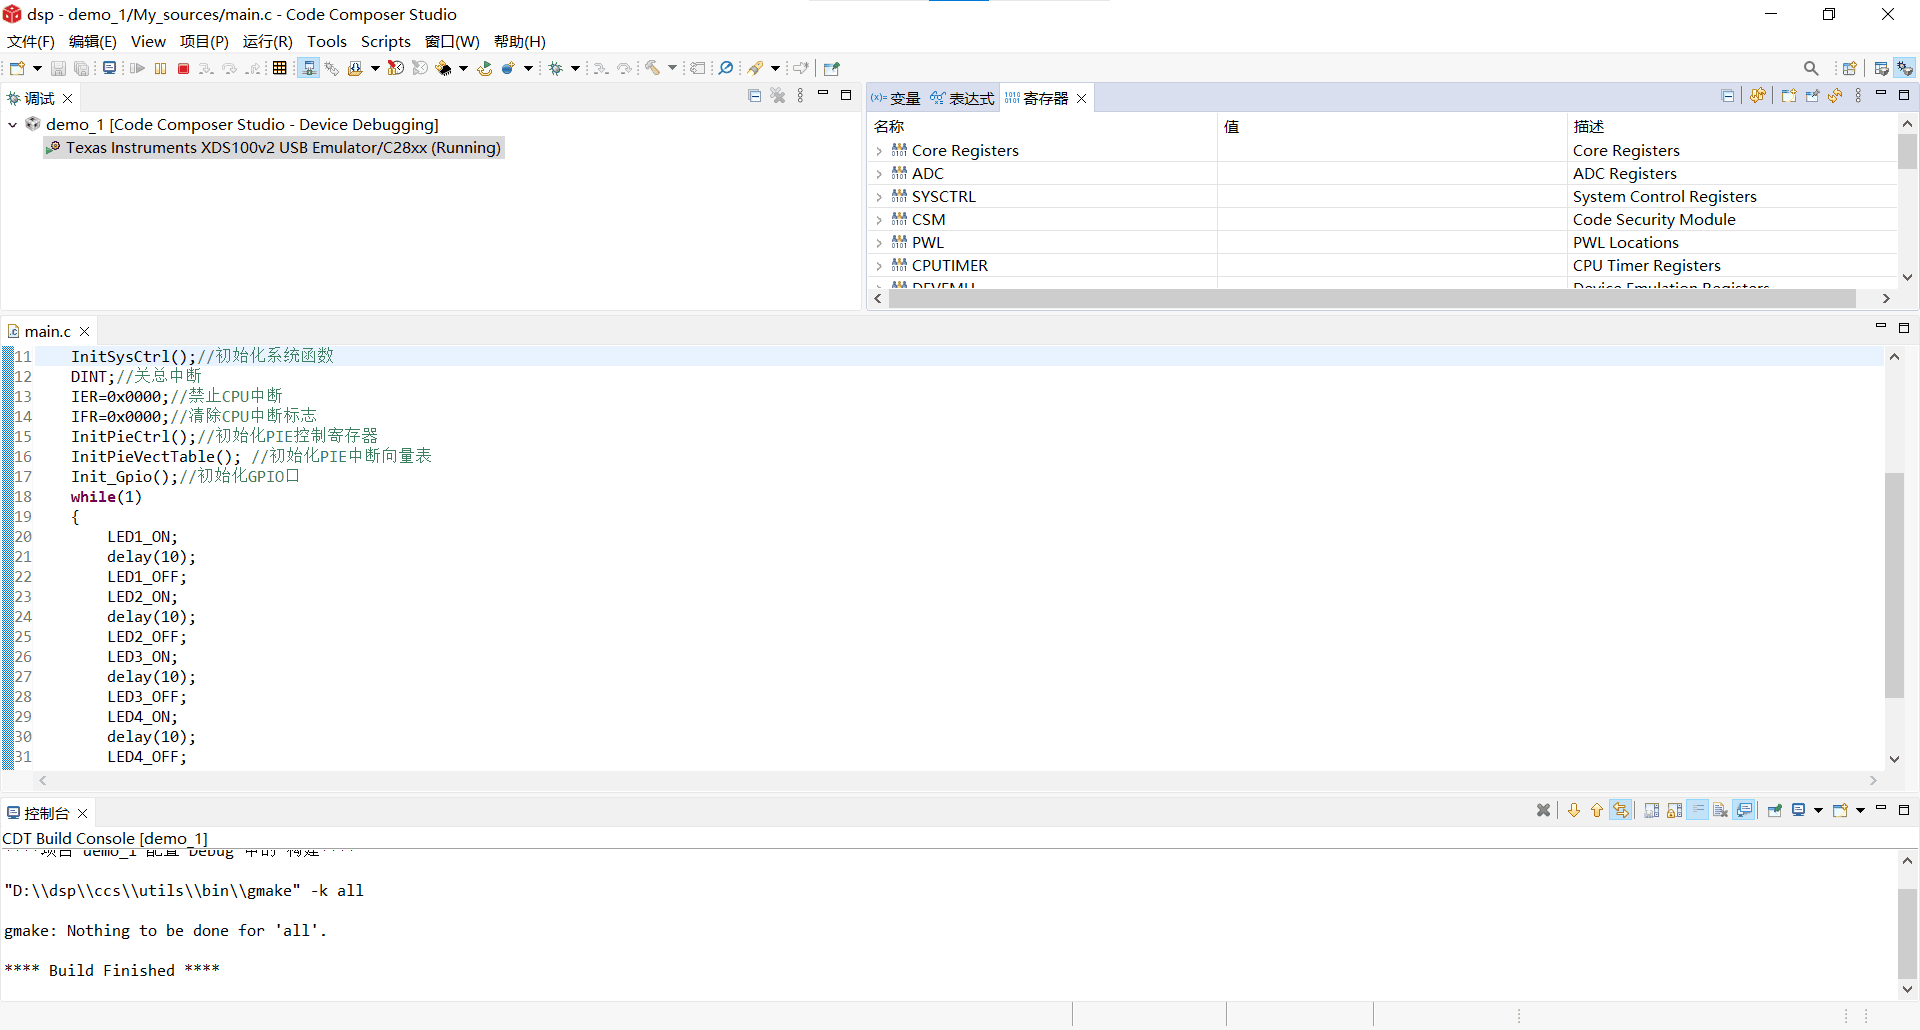
\includegraphics[width=0.8\linewidth]{Picture5.png}  
  \caption{Debug运行}     
\end{figure}

\begin{figure}[H]  
  \centering\includegraphics[width=0.8\linewidth]{Picture6.jpg}  
  \caption{led点亮流水灯}     
\end{figure}

\section{实验小结}

遇到的ERROR汇总

\begin{lstlisting}[frame=single, numbers=left, language=make]
  /Applications/ti/ccs1230/ccs/utils/bin/gmake -k all
  My_sources/Init_Function.d:4: *** target pattern contains no '%'.  Stop
\end{lstlisting}

\end{document}
